\begin{figure}[ht]
\begin{doublespacing}
	\begin{minipage}[b]{0.4\linewidth}
		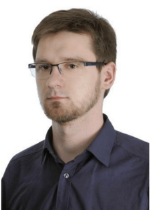
\includegraphics[width=4cm]{img/authors_picture.png}
	\end{minipage}
	\begin{minipage}[b]{0.5\linewidth}
		Kierunek:  Automatyka i Robotyka \\
		Specjalność:  Informatyka Przemysłowa \\
		Data urodzenia:  30.01.1993r. \\
		Data rozpoczęcia studiów:  23.02.2016r. \\
	\end{minipage}
	
	\hspace{2cm}
	
	\begin{center}
		\huge{\textbf{Życiorys}} \\
	\end{center}
	

Urodziłem się 30 stycznia 1993 roku w Zgierzu. W 2012 roku rozpocząłem studia inżynierskie I stopnia na Wydziale Mechatroniki Politechniki Warszawskiej, na kierunku Automatyka i Robotyka, specjalność Robotyka. Ukończyłem je 16 lutego 2016 roku z wynikiem bardzo dobrym. Następnie, tego samego roku  rozpocząłem studia II stopnia na tym samym wydziale, na specjalności Informatyka Przemysłowa. \\

	\vspace{2cm}
	\begin{flushright}
				.............................................. \\
	\end{flushright}
\end{doublespacing}
\end{figure}


